% Options for packages loaded elsewhere
\PassOptionsToPackage{unicode}{hyperref}
\PassOptionsToPackage{hyphens}{url}
%
\documentclass[
  12pt,
]{article}
\usepackage[]{mathpazo}
\usepackage{amssymb,amsmath}
\usepackage{ifxetex,ifluatex}
\ifnum 0\ifxetex 1\fi\ifluatex 1\fi=0 % if pdftex
  \usepackage[T1]{fontenc}
  \usepackage[utf8]{inputenc}
  \usepackage{textcomp} % provide euro and other symbols
\else % if luatex or xetex
  \usepackage{unicode-math}
  \defaultfontfeatures{Scale=MatchLowercase}
  \defaultfontfeatures[\rmfamily]{Ligatures=TeX,Scale=1}
\fi
% Use upquote if available, for straight quotes in verbatim environments
\IfFileExists{upquote.sty}{\usepackage{upquote}}{}
\IfFileExists{microtype.sty}{% use microtype if available
  \usepackage[]{microtype}
  \UseMicrotypeSet[protrusion]{basicmath} % disable protrusion for tt fonts
}{}
\makeatletter
\@ifundefined{KOMAClassName}{% if non-KOMA class
  \IfFileExists{parskip.sty}{%
    \usepackage{parskip}
  }{% else
    \setlength{\parindent}{0pt}
    \setlength{\parskip}{6pt plus 2pt minus 1pt}}
}{% if KOMA class
  \KOMAoptions{parskip=half}}
\makeatother
\usepackage{xcolor}
\IfFileExists{xurl.sty}{\usepackage{xurl}}{} % add URL line breaks if available
\IfFileExists{bookmark.sty}{\usepackage{bookmark}}{\usepackage{hyperref}}
\hypersetup{
  pdftitle={CA 4 - Predictive Modelling},
  hidelinks,
  pdfcreator={LaTeX via pandoc}}
\urlstyle{same} % disable monospaced font for URLs
\usepackage[margin=3cm]{geometry}
\usepackage{color}
\usepackage{fancyvrb}
\newcommand{\VerbBar}{|}
\newcommand{\VERB}{\Verb[commandchars=\\\{\}]}
\DefineVerbatimEnvironment{Highlighting}{Verbatim}{commandchars=\\\{\}}
% Add ',fontsize=\small' for more characters per line
\usepackage{framed}
\definecolor{shadecolor}{RGB}{248,248,248}
\newenvironment{Shaded}{\begin{snugshade}}{\end{snugshade}}
\newcommand{\AlertTok}[1]{\textcolor[rgb]{0.94,0.16,0.16}{#1}}
\newcommand{\AnnotationTok}[1]{\textcolor[rgb]{0.56,0.35,0.01}{\textbf{\textit{#1}}}}
\newcommand{\AttributeTok}[1]{\textcolor[rgb]{0.77,0.63,0.00}{#1}}
\newcommand{\BaseNTok}[1]{\textcolor[rgb]{0.00,0.00,0.81}{#1}}
\newcommand{\BuiltInTok}[1]{#1}
\newcommand{\CharTok}[1]{\textcolor[rgb]{0.31,0.60,0.02}{#1}}
\newcommand{\CommentTok}[1]{\textcolor[rgb]{0.56,0.35,0.01}{\textit{#1}}}
\newcommand{\CommentVarTok}[1]{\textcolor[rgb]{0.56,0.35,0.01}{\textbf{\textit{#1}}}}
\newcommand{\ConstantTok}[1]{\textcolor[rgb]{0.00,0.00,0.00}{#1}}
\newcommand{\ControlFlowTok}[1]{\textcolor[rgb]{0.13,0.29,0.53}{\textbf{#1}}}
\newcommand{\DataTypeTok}[1]{\textcolor[rgb]{0.13,0.29,0.53}{#1}}
\newcommand{\DecValTok}[1]{\textcolor[rgb]{0.00,0.00,0.81}{#1}}
\newcommand{\DocumentationTok}[1]{\textcolor[rgb]{0.56,0.35,0.01}{\textbf{\textit{#1}}}}
\newcommand{\ErrorTok}[1]{\textcolor[rgb]{0.64,0.00,0.00}{\textbf{#1}}}
\newcommand{\ExtensionTok}[1]{#1}
\newcommand{\FloatTok}[1]{\textcolor[rgb]{0.00,0.00,0.81}{#1}}
\newcommand{\FunctionTok}[1]{\textcolor[rgb]{0.00,0.00,0.00}{#1}}
\newcommand{\ImportTok}[1]{#1}
\newcommand{\InformationTok}[1]{\textcolor[rgb]{0.56,0.35,0.01}{\textbf{\textit{#1}}}}
\newcommand{\KeywordTok}[1]{\textcolor[rgb]{0.13,0.29,0.53}{\textbf{#1}}}
\newcommand{\NormalTok}[1]{#1}
\newcommand{\OperatorTok}[1]{\textcolor[rgb]{0.81,0.36,0.00}{\textbf{#1}}}
\newcommand{\OtherTok}[1]{\textcolor[rgb]{0.56,0.35,0.01}{#1}}
\newcommand{\PreprocessorTok}[1]{\textcolor[rgb]{0.56,0.35,0.01}{\textit{#1}}}
\newcommand{\RegionMarkerTok}[1]{#1}
\newcommand{\SpecialCharTok}[1]{\textcolor[rgb]{0.00,0.00,0.00}{#1}}
\newcommand{\SpecialStringTok}[1]{\textcolor[rgb]{0.31,0.60,0.02}{#1}}
\newcommand{\StringTok}[1]{\textcolor[rgb]{0.31,0.60,0.02}{#1}}
\newcommand{\VariableTok}[1]{\textcolor[rgb]{0.00,0.00,0.00}{#1}}
\newcommand{\VerbatimStringTok}[1]{\textcolor[rgb]{0.31,0.60,0.02}{#1}}
\newcommand{\WarningTok}[1]{\textcolor[rgb]{0.56,0.35,0.01}{\textbf{\textit{#1}}}}
\usepackage{longtable,booktabs}
% Correct order of tables after \paragraph or \subparagraph
\usepackage{etoolbox}
\makeatletter
\patchcmd\longtable{\par}{\if@noskipsec\mbox{}\fi\par}{}{}
\makeatother
% Allow footnotes in longtable head/foot
\IfFileExists{footnotehyper.sty}{\usepackage{footnotehyper}}{\usepackage{footnote}}
\makesavenoteenv{longtable}
\usepackage{graphicx}
\makeatletter
\def\maxwidth{\ifdim\Gin@nat@width>\linewidth\linewidth\else\Gin@nat@width\fi}
\def\maxheight{\ifdim\Gin@nat@height>\textheight\textheight\else\Gin@nat@height\fi}
\makeatother
% Scale images if necessary, so that they will not overflow the page
% margins by default, and it is still possible to overwrite the defaults
% using explicit options in \includegraphics[width, height, ...]{}
\setkeys{Gin}{width=\maxwidth,height=\maxheight,keepaspectratio}
% Set default figure placement to htbp
\makeatletter
\def\fps@figure{htbp}
\makeatother
\setlength{\emergencystretch}{3em} % prevent overfull lines
\providecommand{\tightlist}{%
  \setlength{\itemsep}{0pt}\setlength{\parskip}{0pt}}
\setcounter{secnumdepth}{-\maxdimen} % remove section numbering
\usepackage{titling}
\usepackage{pdfpages}
\usepackage{atbegshi}% http://ctan.org/pkg/atbegshi
\usepackage{threeparttable}
\usepackage{multirow}
\usepackage{booktabs}
\usepackage{float}
\usepackage{ragged2e}
\usepackage{tabularx}

\AtBeginDocument{\AtBeginShipoutNext{\AtBeginShipoutDiscard}}
\pretitle{%
  \begin{center}
  \LARGE
  
\includepdf[pages=-]{cover_sheet.pdf}
}
\posttitle{\end{center}}
\usepackage{booktabs}
\usepackage{longtable}
\usepackage{array}
\usepackage{multirow}
\usepackage{wrapfig}
\usepackage{float}
\usepackage{colortbl}
\usepackage{pdflscape}
\usepackage{tabu}
\usepackage{threeparttable}
\usepackage{threeparttablex}
\usepackage[normalem]{ulem}
\usepackage{makecell}
\usepackage{xcolor}
\newlength{\cslhangindent}
\setlength{\cslhangindent}{1.5em}
\newenvironment{cslreferences}%
  {\setlength{\parindent}{0pt}%
  \everypar{\setlength{\hangindent}{\cslhangindent}}\ignorespaces}%
  {\par}

\title{CA 4 - Predictive Modelling}
\usepackage{etoolbox}
\makeatletter
\providecommand{\subtitle}[1]{% add subtitle to \maketitle
  \apptocmd{\@title}{\par {\large #1 \par}}{}{}
}
\makeatother
\subtitle{Health in Ireland}
\author{}
\date{\vspace{-2.5em}}

\begin{document}
\maketitle

\setcounter{page}{1}
\renewcommand{\arraystretch}{1.5}
\renewcommand{\footnotesize}{\small \justify}

\begingroup
\setlength{\tabcolsep}{15pt} 
\renewcommand{\arraystretch}{1.5} 
  \begin{tabular}[]{@{}ll@{}}
    \bf Title:      & Forecasting Saolta University Hospital Group Waiting List Figures \\
    \bf Author:     & Danny Regan \\
    \bf Supervisor: & Dr James Connolly \\
    \bf Degree:     & MSc in Big Data Analytics \\
    \bf Module:     & Data Science \\
    \bf Github:     & \url{https://github.com/ancodia/hospital_waiting_lists}
  \end{tabular}
\endgroup

\hypertarget{abstract}{%
\section{Abstract}\label{abstract}}

This project aims to determine how accurately waiting list figures for the Saolta University Hospital Group can be forecasted through predictive modelling. Time series forecasting with ARIMA modelling was chosen as the method to use for predictions due to the time-based nature of the source data. ARIMA(1,1,0) with drift included was found to offer the greatest accuracy levels after comparison of all model configurations implemented.

A correlation accuracy of 83\% was found between the actual values and those predicted with the ARIMA(1,1,0) with drift model which implies a high level of confidence in the accuracy of predictions. This ARIMA configuration was then used to forecast monthly waiting list totals for 2020. A mean percentage increase of 3.2\% was found between the actual totals from 2019 and those forecasted for 2020, indicating that the increasing trend in the data is likely to continue upwards.

\newpage

\hypertarget{introduction}{%
\section{Introduction}\label{introduction}}

The volume of patients waiting for hospital procedures and the length of these waits constitute a major shortfall in the Irish public healthcare system. According to the most recent Euro Health Consumer Index (Health Consumer Powerhouse \protect\hyperlink{ref-health_consumer_powerhouse_euro_2018}{2018}, p.15), Ireland has the longest waiting times in Europe despite having one of the greatest levels of expenditure on health (OECD and European Union \protect\hyperlink{ref-oecd_health_2018}{2018}, p.133).

The National Treatment Purchase Fund (NTPF) is the organisation assigned the task by the Irish government of collecting, collating and validating data about individuals who are waiting for treatment in public hospitals. This is the source of data for the current project. The objective of this project is to apply predictive modelling to the NTPF waiting list data, evaluate its accuracy and forecast future numbers of patients waiting for hospital procedures. The Saolta University Hospital Group which hospitals in the west and north-west of Ireland will be the subject of this experimentation.

The next section (\hyperref[sec:selection]{Predictive Model Selection}) of this document covers the model selection process including justification through analysis and visualisations. Following that in the \hyperref[sec:build-eval]{Build and Evaluate Predictive Model} section is a discussion around the construction and evaluation of the selected predictive model configurations. The accuracy of the forecast returned by the models is documented and the best performing one is identified in the section called \hyperref[sec:validation]{Model Validation}. Finally in the \hyperref[sec:forecasting]{Model Forecasting and Appraisal} section, the chosen model is used to predict future waiting list numbers for the Saolta group and these are compared to the latest year from the source data. All R code referenced in this document is found in \texttt{predictive\_modelling/time\_series\_predictions.R} which can be accessed in the Github repository listed on the cover page.

\hypertarget{research-question}{%
\subsubsection{Research Question}\label{research-question}}

The NTPF waiting list data will be used in this project to answer the following research question:

\begin{quote}
How accurately can waiting list figures for the Saolta University Hospital Group be forecasted using predictive modelling?
\end{quote}

\hypertarget{predictive-model-selection}{%
\section{Predictive Model Selection}\label{predictive-model-selection}}

\label{sec:selection}
Time series forecasting is the most suitable method for predictive modelling on the waiting list due to its time-based nature. The monthly totals of patients waiting for hospital procedures are the main point of interest and autoregressive integrated moving average (ARIMA) modelling is fit for this task. This section discusses the preparation of waiting list data for the Saolta University Hospital Group for predictive modelling and includes analysis of the constitution of the data to determine what type of ARIMA model should be implemented.

The combined waiting list data that was created during CA3 is loaded and records for the Saolta University Hospital group extracted from it. The day part of the archive date variable is excluded so that it can be guaranteed that only one record per month is in the resulting dataset. Monthly waiting list totals are then aggregated and the number of rows present is now 72 as expected - 12 months x 6 years (2014-19).
\small

\begin{Shaded}
\begin{Highlighting}[]
\NormalTok{waiting\_lists \textless{}{-}}\StringTok{ }\KeywordTok{read\_csv}\NormalTok{(}\StringTok{"data\_prep/combined\_waiting\_lists.csv"}\NormalTok{)}

\NormalTok{saolta \textless{}{-}}\StringTok{ }\KeywordTok{subset}\NormalTok{(waiting\_lists, Hospital\_Group }\OperatorTok{==}\StringTok{ "Saolta"}\NormalTok{)}

\NormalTok{saolta}\OperatorTok{$}\NormalTok{Archive\_Date \textless{}{-}}\StringTok{ }\KeywordTok{format}\NormalTok{(}\KeywordTok{as.Date}\NormalTok{(saolta}\OperatorTok{$}\NormalTok{Archive\_Date, }
                                      \DataTypeTok{format=}\StringTok{"\%Y{-}\%m{-}\%d"}\NormalTok{), }
                              \StringTok{"\%Y{-}\%m"}\NormalTok{)}

\NormalTok{saolta \textless{}{-}}\StringTok{ }\KeywordTok{aggregate}\NormalTok{(}\KeywordTok{cbind}\NormalTok{(Total) }\OperatorTok{\textasciitilde{}}\StringTok{ }
\StringTok{                      }\NormalTok{Archive\_Date, }
                    \DataTypeTok{data =}\NormalTok{ saolta, sum)}
\KeywordTok{nrow}\NormalTok{(saolta)}
\end{Highlighting}
\end{Shaded}

\begin{verbatim}
## [1] 72
\end{verbatim}

\normalsize

To facilitate ARIMA forecasting, the waiting list data is converted to a time series object. A frequency parameter of 12 is used because the time points found in the source data are monthly and the series is set to begin from January 2014. The content of the time series can be seen in Table \ref{tab:ts-table} below.

\begin{Shaded}
\begin{Highlighting}[]
\NormalTok{saolta\_ts \textless{}{-}}\StringTok{ }\KeywordTok{ts}\NormalTok{(saolta}\OperatorTok{$}\NormalTok{Total, }\DataTypeTok{frequency =} \DecValTok{12}\NormalTok{, }\DataTypeTok{start =} \KeywordTok{c}\NormalTok{(}\DecValTok{2014}\NormalTok{, }\DecValTok{1}\NormalTok{))}
\end{Highlighting}
\end{Shaded}

\begin{table}[ht]
\centering
\begingroup\fontsize{7.5pt}{8pt}\selectfont
\begin{tabularx}{\textwidth}{rrrrrrrrrrrrr}
  \hline
 & Jan & Feb & Mar & Apr & May & Jun & Jul & Aug & Sep & Oct & Nov & Dec \\ 
  \hline
2014 & 64351 & 70105 & 71743 & 73760 & 74442 & 73853 & 75933 & 77240 & 78870 & 79422 & 81328 & 87585 \\ 
  2015 & 88784 & 90709 & 92611 & 94974 & 94446 & 92477 & 92487 & 93211 & 92076 & 90953 & 85676 & 82791 \\ 
  2016 & 84328 & 85118 & 86299 & 88091 & 89099 & 89885 & 90962 & 91652 & 92290 & 92636 & 93437 & 94542 \\ 
  2017 & 95784 & 96980 & 98626 & 100604 & 101702 & 102839 & 104249 & 105063 & 105096 & 105082 & 105101 & 105939 \\ 
  2018 & 105221 & 104076 & 104741 & 104804 & 104832 & 104788 & 104863 & 105064 & 104547 & 105052 & 105510 & 104987 \\ 
  2019 & 107203 & 110075 & 110833 & 111803 & 112612 & 114542 & 115328 & 116622 & 116588 & 115910 & 115755 & 114253 \\ 
   \hline
\end{tabularx}
\endgroup
\caption{Saolta waiting lists time series.} 
\label{tab:ts-table}
\end{table}

There are values for each month so no additional effort is required for cleaning the time series. Figure \ref{fig:ts-plot} features a plot of the time series. The time series is additive due to the consistent growth with no dramatic spikes in the peaks and troughs. The plot shows signs of an upward trend which needs to be investigated further and removed before deciding on which ARIMA model parameters to use. This is handled in the next section. The \texttt{graphics::abline()} function provides the straight line in the chart and indicates that the data has quite a strong linear relationship between numbers of patients waiting and time.

\begin{figure}

{\centering 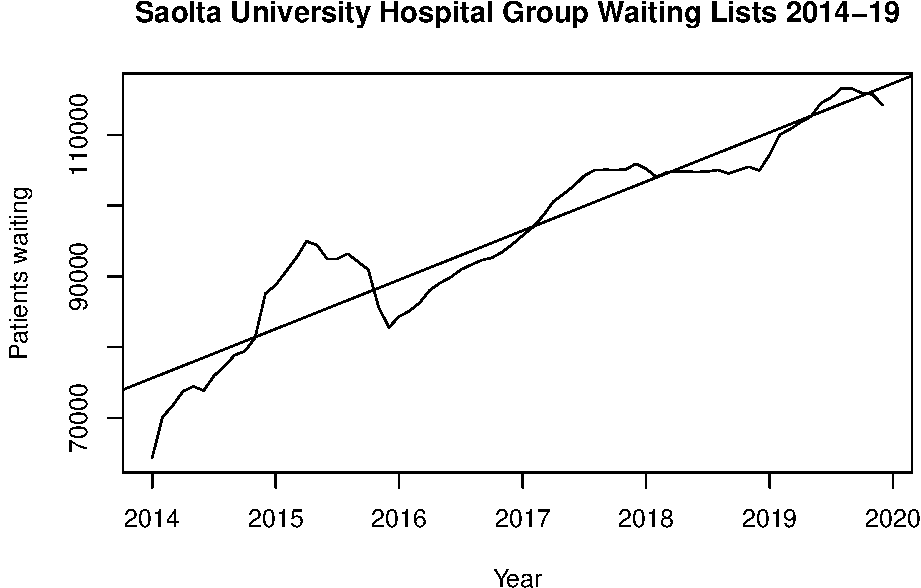
\includegraphics[width=0.8\linewidth]{data_science_ca4_files/figure-latex/ts-plot-1} 

}

\caption{Plot of waiting list time series.}\label{fig:ts-plot}
\end{figure}

A visual check for seasonality can be achieved with a box plot of the cycles contained in the time series (Figure \ref{fig:boxplot}). The median monthly value remains reasonably consistent throughout meaning that no strong link between total number of patients on waiting lists and the time of year is present. Statistical validation of this is featured in the next \hyperref[sec:build-eval]{section} of this document.

\begin{figure}

{\centering 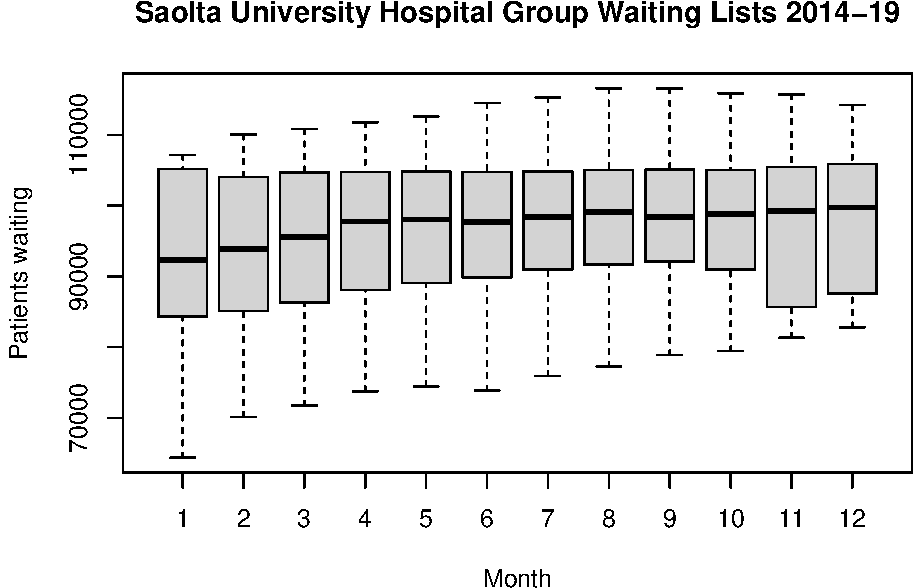
\includegraphics[width=0.8\linewidth]{data_science_ca4_files/figure-latex/boxplot-1} 

}

\caption{Box plot of waiting list time series.}\label{fig:boxplot}
\end{figure}

\hypertarget{build-and-evaluate-predictive-model}{%
\section{Build and Evaluate Predictive Model}\label{build-and-evaluate-predictive-model}}

\label{sec:build-eval}
This section discusses the steps taken in determining the appropriate parameters to use for ARIMA modelling of the time series data and the construction and evaluation of the resulting models. To build a non-seasonal ARIMA model the following values are required:

\begin{itemize}
\item
  \texttt{p}: the number of autoregressive terms from the autocorrelation function (ACF) - AR order.
\item
  \texttt{d}: the number of non-seasonal differences needed to make the time series stationary.
\item
  \texttt{q}: the number of lagged forecast errors from the partial autocorrelation function (PACF) - MA order.
\end{itemize}

Initially, the value for \texttt{d} will be found by verifying that the assumption of non-seasonality is true and then applying differencing to the time series to introduce stationarity. The \texttt{p} and \texttt{q} values are found by plotting the ACF and PACF of the stationary time series respectively.

\hypertarget{stationarity-and-seasonality}{%
\subsection{Stationarity and Seasonality}\label{stationarity-and-seasonality}}

Although the decomposed time series plot (Figure \ref{fig:decomposed-ts}) appears to reveal seasonality in the data, the box plot of the series (Figure \ref{fig:boxplot}) tells otherwise.

\begin{figure}

{\centering 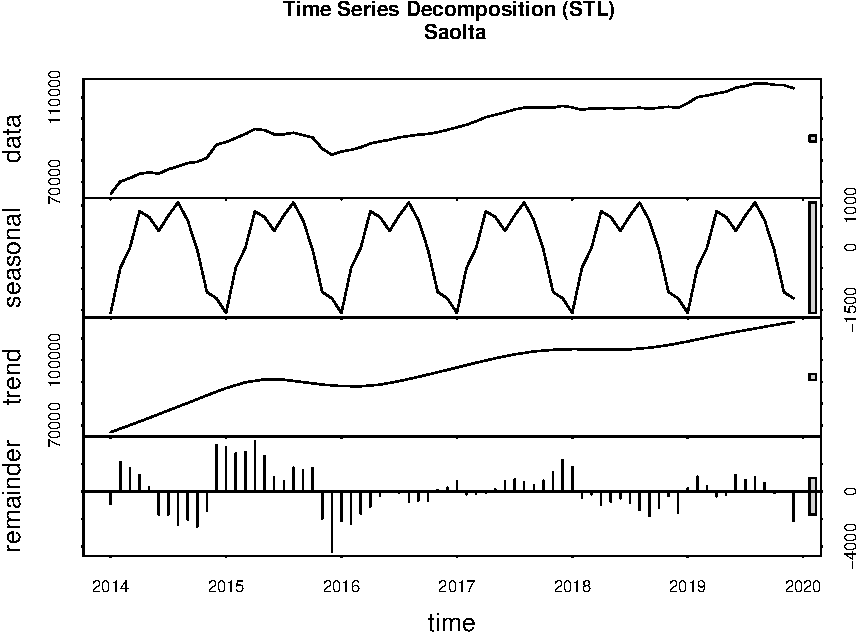
\includegraphics[width=0.8\linewidth]{data_science_ca4_files/figure-latex/decomposed-ts-1} 

}

\caption{Decomposed time series.}\label{fig:decomposed-ts}
\end{figure}

The proportion of variance that each element in the time series makes up can help to determine if there is a higher level of seasonality than expected:
\small

\begin{Shaded}
\begin{Highlighting}[]
\KeywordTok{apply}\NormalTok{(saolta\_ts\_decomposed}\OperatorTok{$}\NormalTok{time.series, }\DecValTok{2}\NormalTok{, var) }\OperatorTok{/}\StringTok{ }\KeywordTok{var}\NormalTok{(saolta\_ts)}
\end{Highlighting}
\end{Shaded}

\begin{verbatim}
##   seasonal      trend  remainder 
## 0.00458736 0.97523453 0.01495276
\end{verbatim}

\normalsize

Seasonality explains only 0.005\% of variance in the time series, confirming the assumption of the lack thereof. The \texttt{seastests::isSeasonal()} function also offers a method of checking for seasonality and returns false as anticipated:
\small

\begin{Shaded}
\begin{Highlighting}[]
\NormalTok{seastests}\OperatorTok{::}\KeywordTok{isSeasonal}\NormalTok{(saolta\_ts)}
\end{Highlighting}
\end{Shaded}

\begin{verbatim}
## [1] FALSE
\end{verbatim}

\normalsize

Trend accounts for almost all variance in the time series so it needs to be removed to make the data stationary and enable ARIMA modelling. Non-stationarity can be visualised by plotting the autocorrelation function (ACF) applied to the data, see Figure \ref{fig:acf-nodiff}. The slow drop off towards 0 seen in the ACF plot demonstrates that the data is not stationary. The ACF of a stationary time series will drop quickly. Differencing must be applied to the data to get it into a stationary form.

\begin{figure}

{\centering 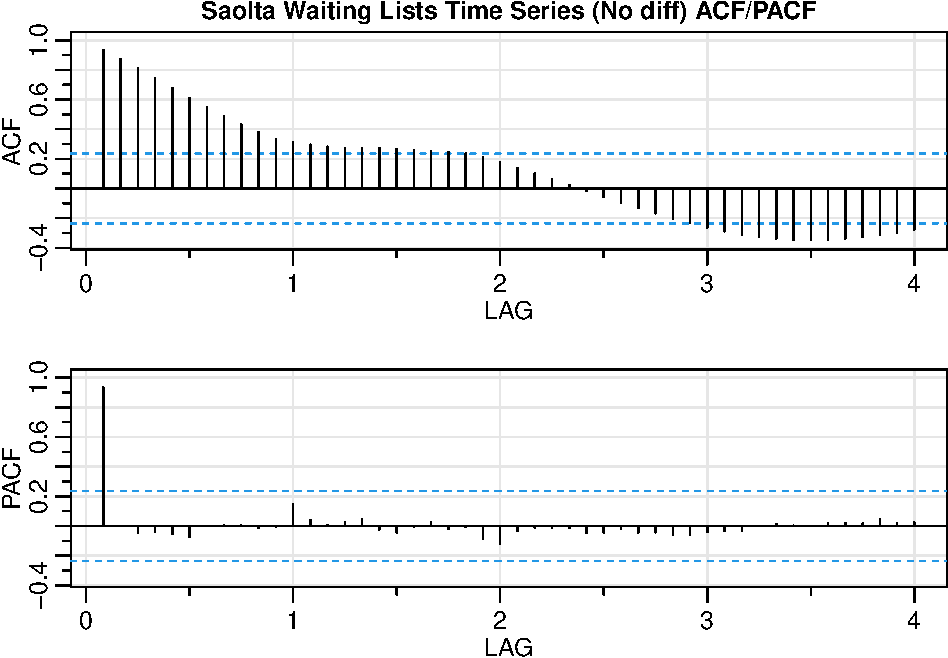
\includegraphics[width=0.8\linewidth]{data_science_ca4_files/figure-latex/acf-nodiff-1} 

}

\caption{ACF/PACF plots of the time series before differencing.}\label{fig:acf-nodiff}
\end{figure}

\hypertarget{find-the-arima-d-value}{%
\subsubsection{Find the ARIMA d value}\label{find-the-arima-d-value}}

Differencing must be applied to the time series to make it stationary, the ARIMA \texttt{d} value is the number of differences required. The \texttt{forecast::ndiffs()} function returns an estimation of how many times differencing should be applied for stationarity to be introduced. In this case, one difference is the value returned:
\small

\begin{Shaded}
\begin{Highlighting}[]
\KeywordTok{ndiffs}\NormalTok{(saolta\_ts)}
\end{Highlighting}
\end{Shaded}

\begin{verbatim}
## [1] 1
\end{verbatim}

\normalsize

To apply differencing to the time series, the \texttt{diff()} function is applied:
\small

\begin{Shaded}
\begin{Highlighting}[]
\NormalTok{saolta\_ts\_diff \textless{}{-}}\StringTok{ }\KeywordTok{diff}\NormalTok{(saolta\_ts, }\DataTypeTok{differences =} \DecValTok{1}\NormalTok{)}
\end{Highlighting}
\end{Shaded}

\normalsize

\newpage

The plot of the differenced time series is shown in Figure \ref{fig:ts-diffed} and appears to be stationary. Running \texttt{ndiffs()} on the differenced time series now shows that no more differences are necessary for stationarity:
\small

\begin{Shaded}
\begin{Highlighting}[]
\KeywordTok{ndiffs}\NormalTok{(saolta\_ts\_diff)}
\end{Highlighting}
\end{Shaded}

\begin{verbatim}
## [1] 0
\end{verbatim}

\normalsize
\begin{figure}

{\centering 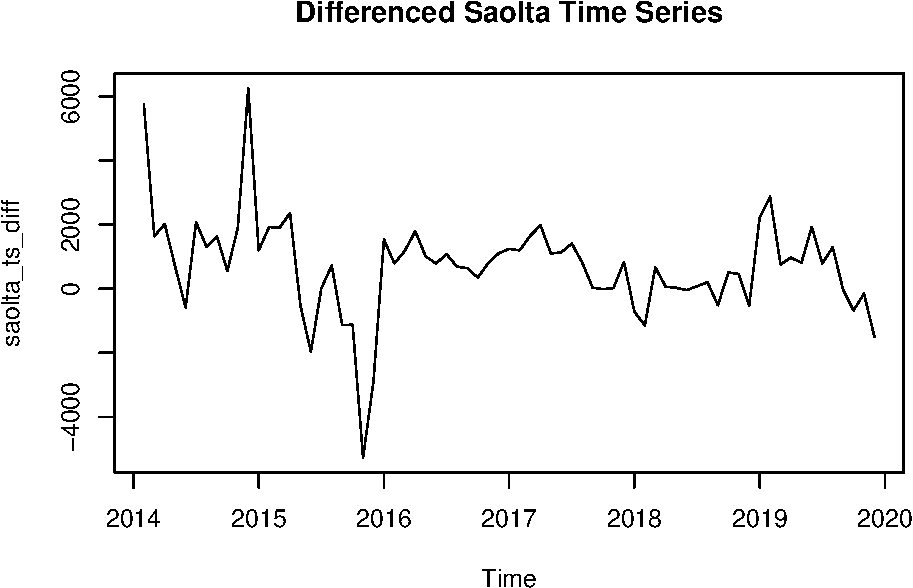
\includegraphics[width=0.8\linewidth]{data_science_ca4_files/figure-latex/ts-diffed-1} 

}

\caption{Differenced time series.}\label{fig:ts-diffed}
\end{figure}

To verify that the time series is now stationary, the Augmented Dickey-Fuller (ADF) and Kwiatkowski-Phillips-Schmidt-Shin (KPSS) tests are applied. The \(H_0\) for ADF is that the time series is not stationary, while \(H_0\) for KPSS is that it is stationary.

ADF (note: using the ADF function from the \texttt{urca} package rather than the \texttt{tseries} version as it can be run with including drift/trend (already removed with differencing):
\small

\begin{Shaded}
\begin{Highlighting}[]
\NormalTok{adf\_pvalue \textless{}{-}}\StringTok{ }\NormalTok{urca}\OperatorTok{::}\KeywordTok{ur.df}\NormalTok{(saolta\_ts\_diff)}\OperatorTok{@}\NormalTok{testreg[[}\StringTok{"coefficients"}\NormalTok{]][}\DecValTok{1}\NormalTok{,}\DecValTok{4}\NormalTok{]}
\NormalTok{adf\_pvalue}
\end{Highlighting}
\end{Shaded}

\begin{verbatim}
## [1] 0.0002702675
\end{verbatim}

\normalsize

p-value is 0.00027 so the null hypothesis of non-stationarity can be rejected.

\newpage

KPSS:
\small

\begin{Shaded}
\begin{Highlighting}[]
\NormalTok{kpss \textless{}{-}}\StringTok{ }\NormalTok{tseries}\OperatorTok{::}\KeywordTok{kpss.test}\NormalTok{(saolta\_ts\_diff)}
\end{Highlighting}
\end{Shaded}

\begin{verbatim}
## Warning in tseries::kpss.test(saolta_ts_diff): p-value greater than printed p-
## value
\end{verbatim}

\begin{Shaded}
\begin{Highlighting}[]
\NormalTok{kpss}\OperatorTok{$}\NormalTok{p.value}
\end{Highlighting}
\end{Shaded}

\begin{verbatim}
## [1] 0.1
\end{verbatim}

\normalsize

A p-value of greater than 0.1 means that the null hypothesis cannot be rejected thus confirming that the time series is in a stationary state.

This one required difference gives an optimum \texttt{d} value of 1 for the ARIMA model.

\hypertarget{arima-p-and-q-values-from-acfpacf}{%
\subsubsection{ARIMA p and q values from ACF/PACF}\label{arima-p-and-q-values-from-acfpacf}}

When the ACF and PACF are plotted for the differenced time series (Figure \ref{fig:acf-diffed}), they both quickly drops below the dotted line indicating that the majority of values are not significantly different from 0. The \texttt{p} and \texttt{q} values can now be taken from this plot, both cut off after 1 lag so this is the value assigned to both. Along with the \texttt{d} value of 1, this provides three possible ARIMA(p,d,q) configurations: ARIMA(1,1,0), ARIMA(0,1,1) and ARIMA(1,1,1).

\begin{figure}

{\centering 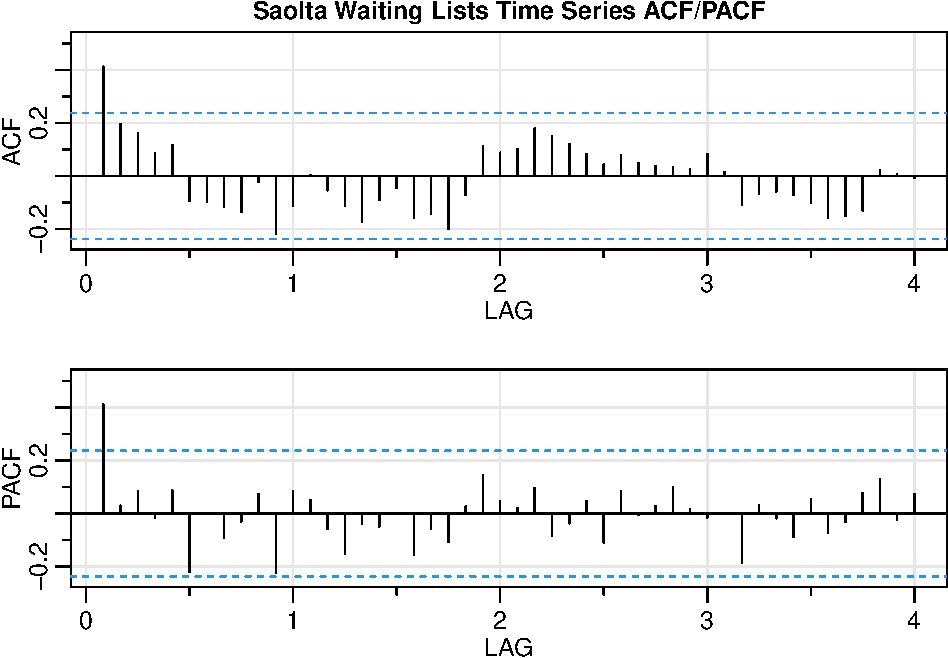
\includegraphics[width=0.8\linewidth]{data_science_ca4_files/figure-latex/acf-diffed-1} 

}

\caption{ACF/PACF plots of the time series after differencing.}\label{fig:acf-diffed}
\end{figure}

\hypertarget{build-models}{%
\subsubsection{Build Models}\label{build-models}}

Using the parameters found above, three ARIMA models will be implemented and \texttt{forecast::auto.arima()} is then used to evaluate if the parameters provided are correct. The original time series must first be split into train and test sets. The training time series includes all cycles from 2014 to 2018, while the test set is made up of all 2019 data.
\small

\begin{Shaded}
\begin{Highlighting}[]
\NormalTok{train \textless{}{-}}\StringTok{ }\KeywordTok{window}\NormalTok{(}\DataTypeTok{x =}\NormalTok{ saolta\_ts, }\DataTypeTok{start =} \KeywordTok{c}\NormalTok{(}\DecValTok{2014}\NormalTok{, }\DecValTok{1}\NormalTok{), }\DataTypeTok{end =} \KeywordTok{c}\NormalTok{(}\DecValTok{2018}\NormalTok{, }\DecValTok{12}\NormalTok{))}
\NormalTok{test \textless{}{-}}\StringTok{ }\KeywordTok{window}\NormalTok{(}\DataTypeTok{x =}\NormalTok{ saolta\_ts, }\DataTypeTok{start =} \KeywordTok{c}\NormalTok{(}\DecValTok{2019}\NormalTok{, }\DecValTok{1}\NormalTok{), }\DataTypeTok{end =} \KeywordTok{c}\NormalTok{(}\DecValTok{2019}\NormalTok{, }\DecValTok{12}\NormalTok{))}
\end{Highlighting}
\end{Shaded}

\normalsize

The training data is used to fit the ARIMA models:
\small

\begin{Shaded}
\begin{Highlighting}[]
\NormalTok{arima\_model1 =}\StringTok{ }\NormalTok{forecast}\OperatorTok{::}\KeywordTok{Arima}\NormalTok{(train, }\DataTypeTok{order =} \KeywordTok{c}\NormalTok{(}\DecValTok{1}\NormalTok{, }\DecValTok{1}\NormalTok{, }\DecValTok{0}\NormalTok{))}
\NormalTok{arima\_model2 =}\StringTok{ }\NormalTok{forecast}\OperatorTok{::}\KeywordTok{Arima}\NormalTok{(train, }\DataTypeTok{order =} \KeywordTok{c}\NormalTok{(}\DecValTok{0}\NormalTok{, }\DecValTok{1}\NormalTok{, }\DecValTok{1}\NormalTok{))}
\NormalTok{arima\_model3 =}\StringTok{ }\NormalTok{forecast}\OperatorTok{::}\KeywordTok{Arima}\NormalTok{(train, }\DataTypeTok{order =} \KeywordTok{c}\NormalTok{(}\DecValTok{1}\NormalTok{, }\DecValTok{1}\NormalTok{, }\DecValTok{1}\NormalTok{))}
\NormalTok{auto\_arima\_model \textless{}{-}}\StringTok{ }\KeywordTok{auto.arima}\NormalTok{(train)}
\end{Highlighting}
\end{Shaded}

\normalsize

The model calculated by \texttt{auto.arima()} is ARIMA(1,1,0) with drift. This drift is the amount of change over time and uses the average change seen in historical data. Drift was not considered during the manual model specification but makes sense with the nature of the time series under investigation. The ARIMA parameters (1,1,0) match that of the first manually specified one, providing additional confidence that the earlier process in determining these parameters was completed correctly. Comparison of these models is the focus of the next section.

\begin{figure}

{\centering 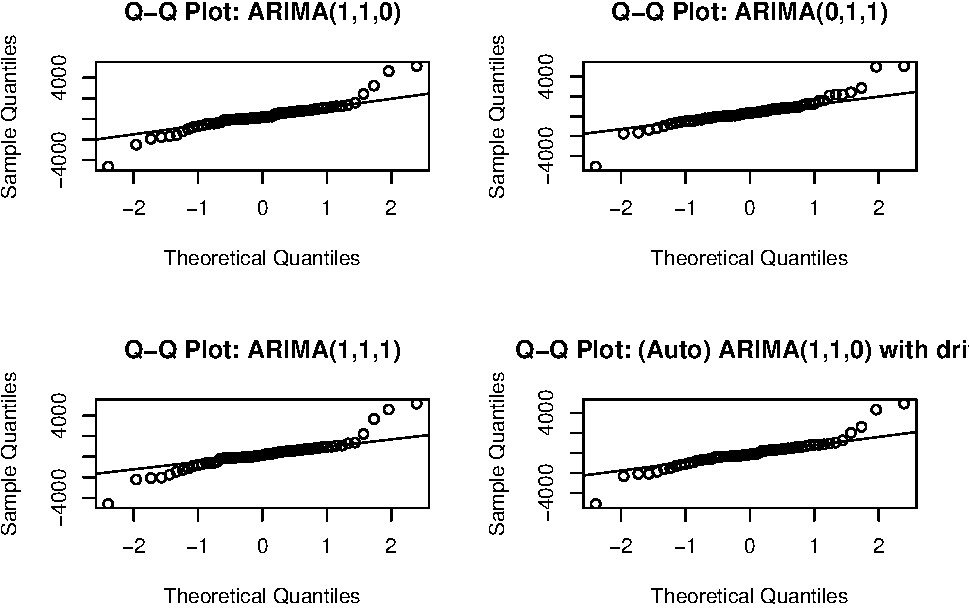
\includegraphics[width=0.8\linewidth]{data_science_ca4_files/figure-latex/qq-plots-1} 

}

\caption{Quantile-Quantile plots for each ARIMA model.}\label{fig:qq-plots}
\end{figure}

\hypertarget{model-validation}{%
\section{Model Validation}\label{model-validation}}

\label{sec:validation}
The following outlines the methods used to evaluate the accuracy of the models proposed in the previous section and determine the best fit for forecasting waiting list totals.

The residuals of each ARIMA model are used to check the models for the presence of normal distributions. Quantile-Quantile plots for each model are featured in Figure \ref{fig:qq-plots} while in Figure \ref{fig:histograms} histograms are the other form of visualisation utilised. From visually inspecting these plots, all implemented ARIMA models appear to be normally distributed. The Ljung-box test which checks for randomness in ARIMA residuals was performed on each set of residuals with p-values recorded in Table \ref{tab:evaluation-metrics}. These are all greater than 0.05 meaning that the residuals are independent of each other which is the anticipated result.

\begin{figure}

{\centering 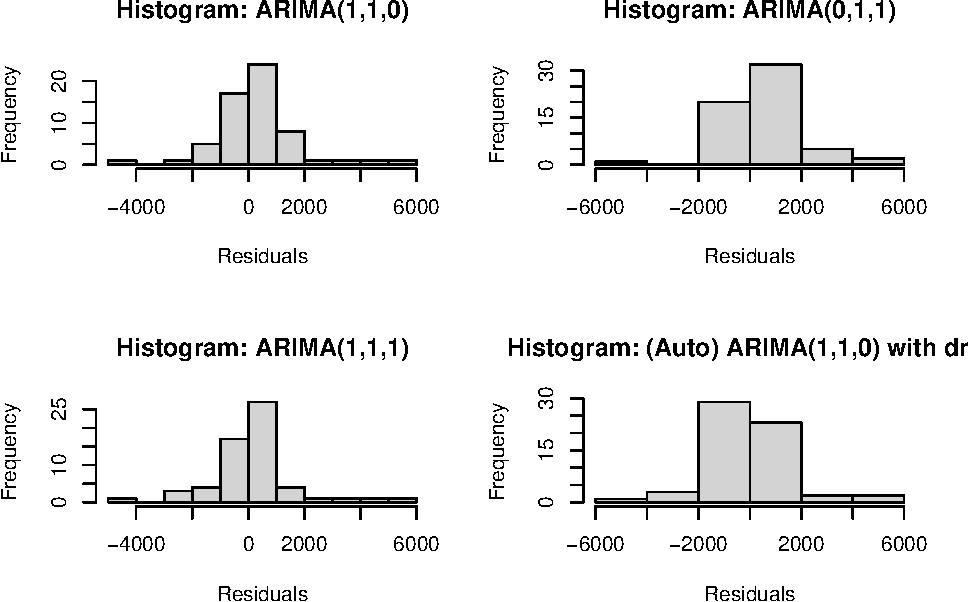
\includegraphics[width=0.8\linewidth]{data_science_ca4_files/figure-latex/histograms-1} 

}

\caption{Histograms for each ARIMA model.}\label{fig:histograms}
\end{figure}

\hypertarget{prediction-accuracy}{%
\subsection{Prediction Accuracy}\label{prediction-accuracy}}

Akaike information criterion (AIC) and the mean absolute percentage error (MAPE) for each of the four models are found in Table \ref{tab:evaluation-metrics}. The \texttt{auto.arima()} generated model (ARIMA(1,1,0) w/ drift) performs best based on both metrics i.e.~it has the lowest score for each. This means this model is expected to have the most accurate predictions.

Predictions for 2019 using each model were calculated with the \texttt{forecast::forecast()} method. Plots for each of these forecasts are displayed in Figure \ref{fig:forecasts}. The ARIMA(1,1,0) w/ drift model's plot looks to be the most accurate due to the inclusion of drift, capturing the general upward growth found in the time series. Whereas each of the other model's mean forecasted values are almost horizontal. The mean forecasted results, as well as the actual figures for each month can be inspected in Table \ref{tab:actuals-preds}.

Correlation accuracy measures for the predictions are listed in Table \ref{tab:corr-accuracy}. All but the model with drift applied were found to be negatively correlated which contradicts the actual waiting list figures for 2019. With these findings, the ARIMA(1,1,0) w/ drift model is selected for forecasting future values in the next section.

\begin{table}

\caption{\label{tab:evaluation-metrics}Evaluation metrics for each implemented ARIMA model.}
\centering
\begin{tabular}[t]{lrrr}
\toprule
Model & AIC & MAPE & Ljung-box\\
\midrule
ARIMA(1,1,0) & 1032.688 & 1.093352 & 0.18205\\
ARIMA(0,1,1) & 1036.507 & 1.135171 & 0.34483\\
ARIMA(1,1,1) & 1034.202 & 1.071500 & 0.49092\\
(Auto) ARIMA(1,1,0) w/ drift & 1031.205 & 1.070920 & 0.52420\\
\bottomrule
\multicolumn{4}{l}{\textsuperscript{} Note: Values listed for Ljung-box are p-values.}\\
\end{tabular}
\end{table}

\begin{figure}

{\centering 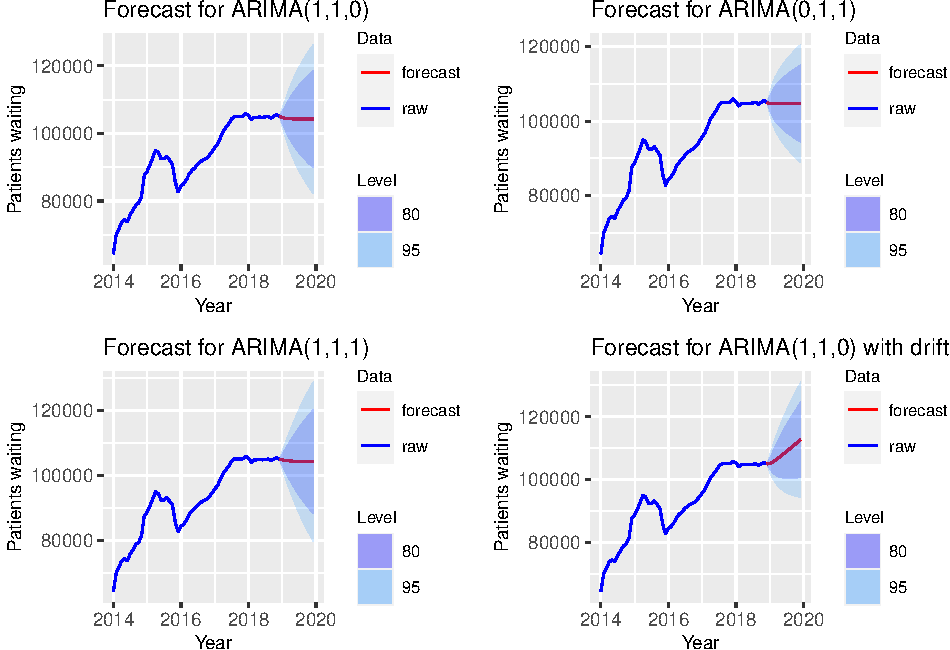
\includegraphics[width=0.9\linewidth]{data_science_ca4_files/figure-latex/forecasts-1} 

}

\caption{Forecast plots for each ARIMA configuration (2019).}\label{fig:forecasts}
\end{figure}

\begin{table}

\caption{\label{tab:actuals-preds}Actual vs Predicted Totals for 2019.}
\centering
\resizebox{\linewidth}{!}{
\begin{tabular}[t]{rrrrrr}
\toprule
2019 & Actual & ARIMA(1,1,0) & ARIMA(0,1,1) & ARIMA(0,1,1) & (Auto) ARIMA(1,1,0)
 w/ drift\\
\midrule
1 & 107203 & 104678.4 & 104694.7 & 104791.9 & 105100.0\\
2 & 110075 & 104496.2 & 104694.7 & 104646.4 & 105531.8\\
3 & 110833 & 104388.8 & 104694.7 & 104537.8 & 106123.3\\
4 & 111803 & 104325.3 & 104694.7 & 104456.8 & 106795.0\\
5 & 112612 & 104287.9 & 104694.7 & 104396.5 & 107506.9\\
\addlinespace
6 & 114542 & 104265.8 & 104694.7 & 104351.4 & 108238.9\\
7 & 115328 & 104252.8 & 104694.7 & 104317.8 & 108981.0\\
8 & 116622 & 104245.1 & 104694.7 & 104292.7 & 109728.1\\
9 & 116588 & 104240.6 & 104694.7 & 104274.0 & 110477.8\\
10 & 115910 & 104237.9 & 104694.7 & 104260.1 & 111228.7\\
\addlinespace
11 & 115755 & 104236.3 & 104694.7 & 104249.7 & 111980.3\\
12 & 114253 & 104235.4 & 104694.7 & 104241.9 & 112732.2\\
\bottomrule
\end{tabular}}
\end{table}

\begin{table}

\caption{\label{tab:corr-accuracy}Actual vs Predicted correlation accuracy for 2019.}
\centering
\resizebox{\linewidth}{!}{
\begin{tabular}[t]{lrrrrr}
\toprule
  & Actual & ARIMA(1,1,0) & ARIMA(0,1,1) & ARIMA(0,1,1).1 & (Auto) ARIMA(1,1,0)
 w/ drift\\
\midrule
Actual & 1.0000000 & -0.9241134 & NA & -0.9545271 & 0.8320844\\
ARIMA(1,1,0) & -0.9241134 & 1.0000000 & NA & 0.9736906 & -0.7855254\\
ARIMA(0,1,1) & NA & NA & 1 & NA & NA\\
ARIMA(0,1,1).1 & -0.9545271 & 0.9736906 & NA & 1.0000000 & -0.8993836\\
(Auto) ARIMA(1,1,0)
 w/ drift & 0.8320844 & -0.7855254 & NA & -0.8993836 & 1.0000000\\
\bottomrule
\end{tabular}}
\end{table}

\newpage

\hypertarget{model-forecasting-and-appraisal}{%
\section{Model Forecasting and Appraisal}\label{model-forecasting-and-appraisal}}

\label{sec:forecasting}
The final stage in this project involves using the most suitable ARIMA model found from the previously performed validation to forecast future waiting list totals for the Saolta University Hospital Group. This forecasting will use the ARIMA(1,1,0) w/ drift model fitted with the entire original time series (2014-19) to predict monthly values for 2020.

The generated forecast is plotted in Figure \ref{fig:forecast2} with the corresponding 2020 forecasted totals compared to 2019 actuals detailed in Table \ref{tab:forecast-2020}. The mean percentage difference when comparing forecasted to actual is 3.202441\%, meaning the model is predicting the upward trend in the number of patients waiting to continue growing. The cycles of the 2019 time series are plotted those from the forecasts for 2020 in Figure \ref{fig:forecast-2020-comparison}, visually representing the predicted difference.

\begin{figure}

{\centering 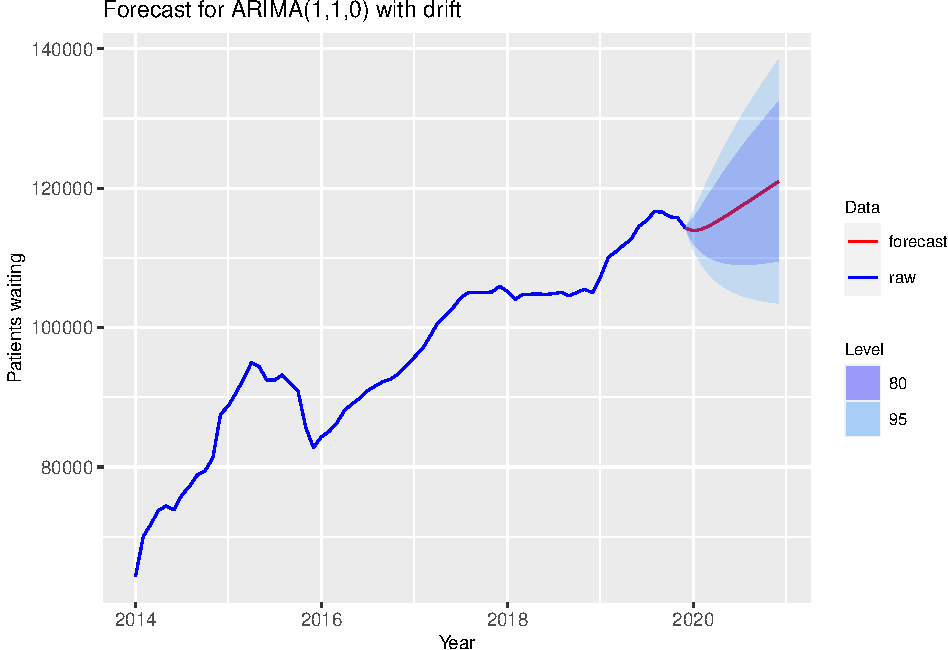
\includegraphics[width=0.7\linewidth]{data_science_ca4_files/figure-latex/forecast2-1} 

}

\caption{Forecast plot for 2020 patient numbers.}\label{fig:forecast2}
\end{figure}

\begin{table}

\caption{\label{tab:forecast-2020}Total Patients waiting monthly - 2019 vs 2020}
\centering
\fontsize{10}{12}\selectfont
\begin{tabular}[t]{rrr}
\toprule
2019 (Actual) & 2020 (Forecasted) & Percentage Change\\
\midrule
107203 & 113889.1 & 6.236863\\
110075 & 114085.8 & 3.643680\\
110833 & 114558.6 & 3.361422\\
111803 & 115167.3 & 3.009173\\
112612 & 115843.1 & 2.869243\\
\addlinespace
114542 & 116551.9 & 1.754703\\
115328 & 117276.9 & 1.689860\\
116622 & 118009.9 & 1.190082\\
116588 & 118746.9 & 1.851695\\
115910 & 119485.8 & 3.084939\\
\addlinespace
115755 & 120225.6 & 3.862130\\
114253 & 120965.9 & 5.875500\\
\bottomrule
\end{tabular}
\end{table}

\begin{figure}

{\centering 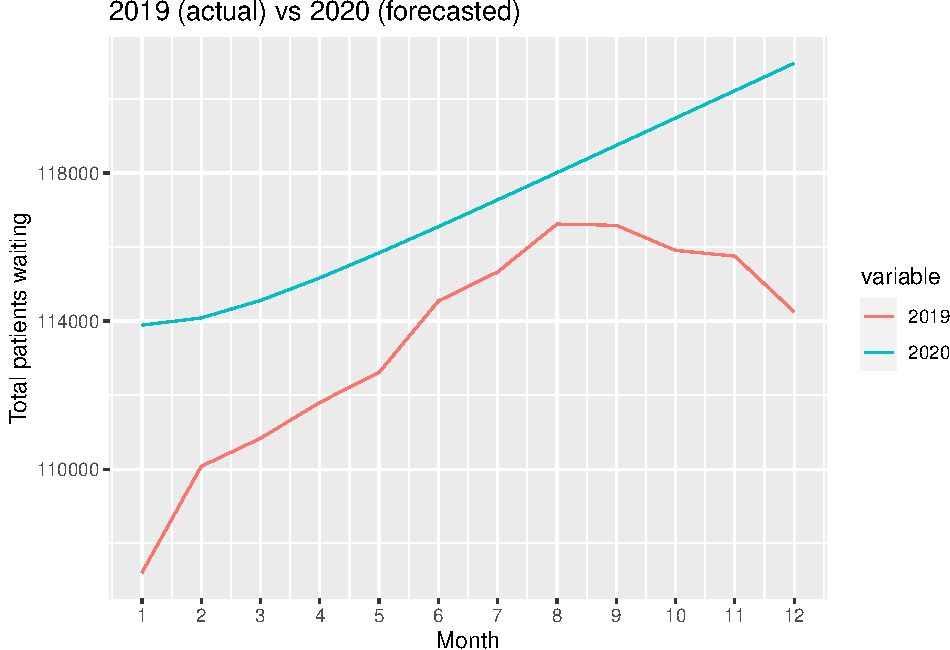
\includegraphics[width=0.8\linewidth]{data_science_ca4_files/figure-latex/forecast-2020-comparison-1} 

}

\caption{2019 (actual) vs 2020 (forecasted).}\label{fig:forecast-2020-comparison}
\end{figure}

\newpage

\hypertarget{conclusions}{%
\section{Conclusions}\label{conclusions}}

The purpose of this project was to determine how accurately waiting list figures for the Saolta University Hospital Group can be forecasted using predictive modelling. ARIMA forecasting was determined to be the best fit for generating predictions from the time-based source data. Inspection of the time series created from the NTPF waiting list data revealed an upward trend but no strong seasonality in the data.

To find the parameters required for proposing ARIMA models, first non-seasonal differencing was applied to the time series to obtain \texttt{d} and \texttt{p} and \texttt{q} values were found by plotting the ACF and PACF applied to the differenced time series. Three models were proposed from these parameters; ARIMA(1,1,0), ARIMA(1,1,1) and ARIMA(0,1,1), while the R \texttt{auto.arima()} function generated a fourth model, ARIMA(1,1,0) w/ drift. Evaluation of the group of models revealed that the automatically generated model provided the lowest level of prediction error and so was determined as the best choice for forecasting future values. The correlation accuracy can be used to answer the stated research question, with the ARIMA(1,1,0) w/ drift model giving a value of 83\% which represents a strong level of prediction accuracy.

Finally, the chosen ARIMA configuration was used to forecast monthly waiting list totals for 2020. The mean percentage increase from 2019 to 2020 was calculated as 3.2\% which if accurate would imply that the upward trend present in the existing data is set to continue to grow.

\hypertarget{references}{%
\section{References}\label{references}}

\hypertarget{refs}{}
\begin{cslreferences}
\leavevmode\hypertarget{ref-health_consumer_powerhouse_euro_2018}{}%
Health Consumer Powerhouse (2018) \emph{Euro Health Consumer Index 2018} {[}online{]}, Health Consumer Powerhouse, available: \url{https://healthpowerhouse.com/media/EHCI-2018/EHCI-2018-report.pdf} {[}accessed 17 Mar 2020{]}.

\leavevmode\hypertarget{ref-oecd_health_2018}{}%
OECD, European Union (2018) \emph{Health at a Glance: Europe 2018: State of Health in the EU Cycle} {[}online{]}, Health at a glance: Europe, OECD, available: \url{https://www.oecd-ilibrary.org/social-issues-migration-health/health-at-a-glance-europe-2018_health_glance_eur-2018-en} {[}accessed 18 Mar 2020{]}.
\end{cslreferences}

\end{document}
